%%%%%%%%%%%%%%%%%%%%%%%%%%%%%%%%%%%%%%%%%%%%%%%%%%%%%%%%%%%%%%%%%%%%%%%%%%%%%%%%%%%
% Team:
% Union
% Members: 
% Bernie Huan, Jim Lan, Hoang Tan, Kenny Hsu, Rahul Aditya, Tan Phat, Wei
% Relative files:
% Main.tex, Background_Union.tex, Library.bib, Union_Background_Chart_1.png, Union_Background_Chart_2.png, Union_Background_Chart_3.png, Union_Background_Chart_semi.png, Union_Background_Chart_sup1.png, Union_Background_Chart_sup2.png, Union_Background_Chart_sup3.png, Union_Background_Chart_WSD.png
% Note:
% Do not compile this file compile Main.tex to get the pdf file instead.
%%%%%%%%%%%%%%%%%%%%%%%%%%%%%%%%%%%%%%%%%%%%%%%%%%%%%%%%%%%%%%%%%%%%%%%%%%%%%%%%%%%

\subsection{Automatic creation of metadata}
\textit{\footnotesize Author:Bernie Huan, Jim Lan, Hoang Tan, Kenny Hsu, Rahul Aditya, Tan Phat, Wei.}\\

We are producing a program that automatically generate and extract metadata with natural language processing. 
We also strive to generate XML files with metadata extracted. 
In the best scenario, we will even try to create a search engine together with other groups. 
Also, creating a sutiable interface and structure with some finctions for users is necessary.  
Following discussion is our literature review on natural language processing.

\begin{figure*}[ht]
	\begin{center}
		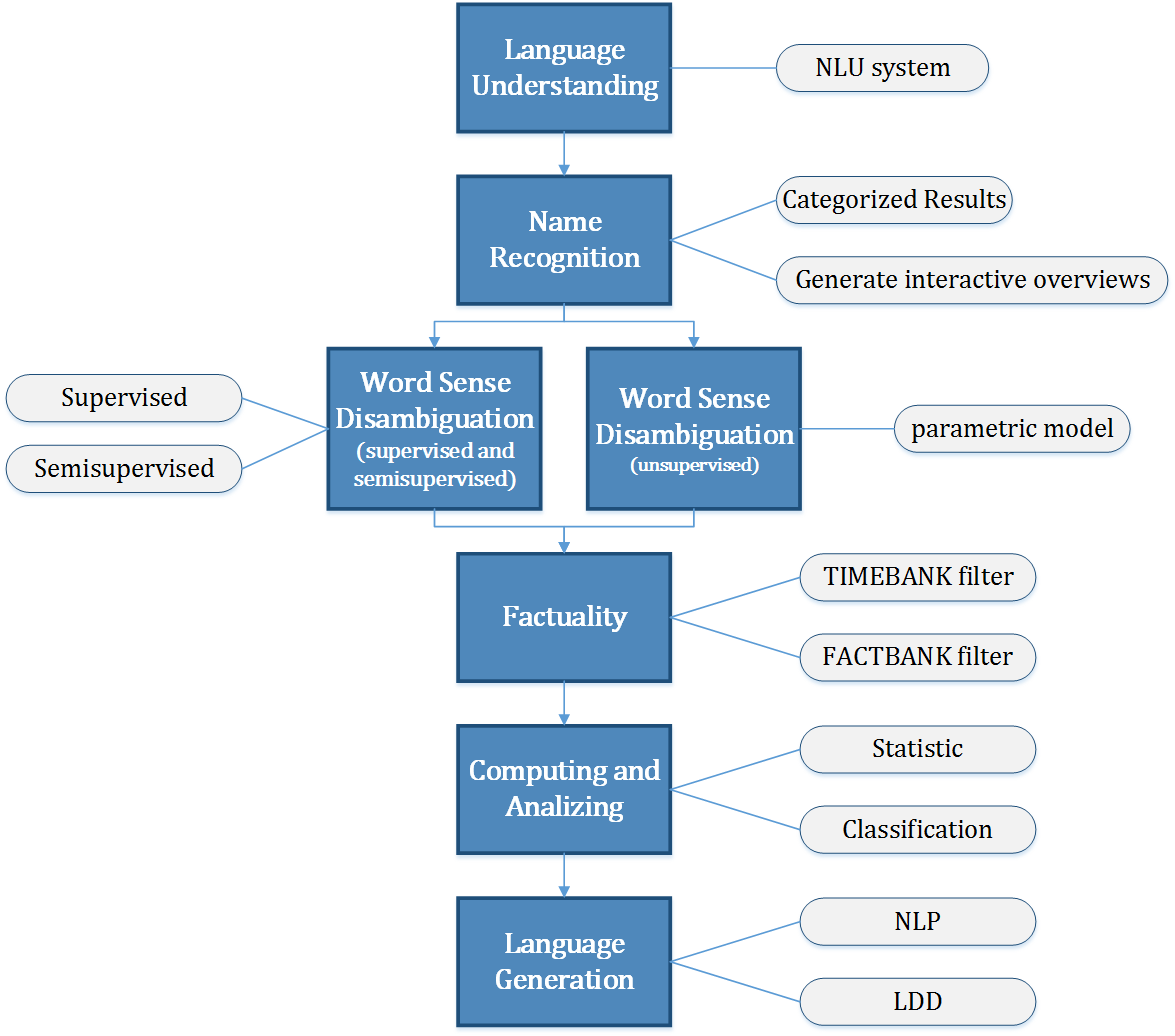
\includegraphics[width=1.8\columnwidth]{Union_Background_Chart_1}
	\end{center}
	\caption{The process of metadata creation.}
\end{figure*}


\subsection{metadata}
\textit{\footnotesize Author:Bernie Huan, Jim Lan, Hoang Tan, Kenny Hsu, Rahul Aditya, Tan Phat, Wei.}\\

We are producing a program that automatically generate and extract metadata with natural language processing. 
We also strive to generate XML files with metadata extracted. 
In the best scenario, we will even try to create a search engine together with other groups. 
Also, creating a sutiable interface and structure with some finctions for users is necessary.  
Following discussion is our literature review on natural language processing.

\begin{figure*}[ht]
	\begin{center}
		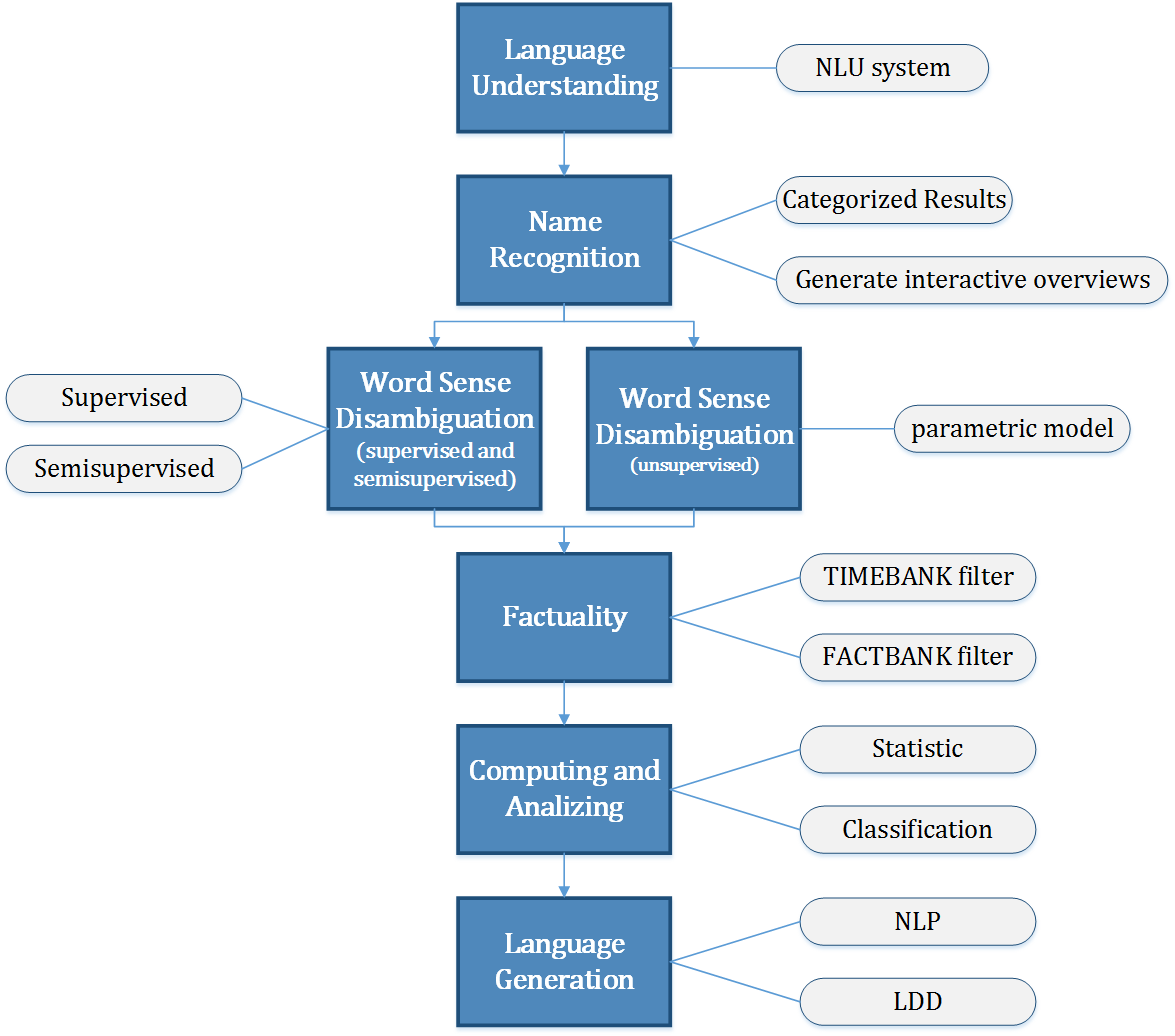
\includegraphics[width=1.8\columnwidth]{Union_Background_Chart_1}
	\end{center}
	\caption{The process of metadata creation.}
\end{figure*}


\subsubsection*{Language understanding}
Natural language understanding (NLU) is a subtopic of natural language processing in artificial intelligence that deals with machine reading comprehension, it's considered an AI-hard problem.

When users search for a sentence, how does the program understand the certain inputs of text? 

We could build a natural language understanding (NLU) system, in which the system's rules for semantic interpretation are 
learnt automatically from training data, which uses a set of possible yes-no questions that can be applied to data items.
After that, it follows rules for selecting the best questions at any node on the basis of training data by using a method for pruning trees to prevent over-training.



\subsubsection*{Language}
Natural language understanding (NLU) is a subtopic of natural language processing in artificial intelligence that deals with machine reading comprehension, it's considered an AI-hard problem.

When users search for a sentence, how does the program understand the certain inputs of text? 

We could build a natural language understanding (NLU) system, in which the system's rules for semantic interpretation are 
learnt automatically from training data, which uses a set of possible yes-no questions that can be applied to data items.
After that, it follows rules for selecting the best questions at any node on the basis of training data by using a method for pruning trees to prevent over-training.


\subsubsection*{Name Recognition}

The results could be a country or an animal if users search for the word, Turkey. The meaning is totally different and
definitely make users very confused if he or she is not very familiar with "Turkey". 

There are a lot of misunderstandings like this if users search some words which have multiply meanings.
Sometimes, the results are fully unrelated and this situation is always annoying. 
That would be troublesome when we count frequency of certain words to rank them.

Therefore, it is significantly crucial for a program to totally understand what users want by name recognition in natural language processing. 
The users can find out the results much quicker and will not be confused.

The method to improve the problem above is "categorize the words based on different subjects,topic or genres" by using online database and python program.
Metadata is limited in digital libraries and web resources, try to enlarge them with meaningful, organized and desired
categories \cite{Kules2006}.

Besides dealing with mutiple-meaning words,the most important part of name recognition is to recognize the special names and terms such as locations,people name,country,even company names and academic terms.
Therefore, it is better for search engine to know what user want and huge name corpus are necessary. Plus, this work also can assist previous work.

With above effort,users' exploration and overviews of information could be better supported. 
It will be very convenient to find the results we want and lower the possibility of misunderstandings if users are not 
very familiar with finding the appropriate result in specific fields.\cite{TunThuraThet2010} 
Users dose not have to filter the results which are ranked by browsing frequency popularity. 
Users just can obtain the information and relevance by clicking the specific categories and some reasonable choices.

Plus,creating some choices for users is also vital because this make the searching much more oragnized.
For example,if there are a lot of subtitles such as abstract, introduction,method or references in some standard research 
articles, try to make some choices so that the users can easily find out what they want.
There are a lot of different standard articles in the world.
Making a suitable choices if someone want to creat a personalzed search engine and interface. 
     
Also, users are able to choose multiply fields if the results include a lot of relevant fields. 
That's a big motivation for people to handle this problems. 

A lot of online services have done similar tasks before.
Thus,creating and using an online databasees or automated metadata creation are to be recommended.
The reason is there are many advantages, including integrating with the other cloud services or scaling with what users 
need such as how to categorize the categories.
It is beneficial for people who would like to create a convenient and personalized database or metadata.\\



\subsubsection*{Title Recognition}

The results could be a country or an animal if users search for the word, Turkey. The meaning is totally different and
definitely make users very confused if he or she is not very familiar with "Turkey". 

There are a lot of misunderstandings like this if users search some words which have multiply meanings.
Sometimes, the results are fully unrelated and this situation is always annoying. 
That would be troublesome when we count frequency of certain words to rank them.

Therefore, it is significantly crucial for a program to totally understand what users want by name recognition in natural language processing. 
The users can find out the results much quicker and will not be confused.

The method to improve the problem above is "categorize the words based on different subjects,topic or genres" by using online database and python program.
Metadata is limited in digital libraries and web resources, try to enlarge them with meaningful, organized and desired
categories \cite{Kules2006}.

Besides dealing with mutiple-meaning words,the most important part of name recognition is to recognize the special names and terms such as locations,people name,country,even company names and academic terms.
Therefore, it is better for search engine to know what user want and huge name corpus are necessary. Plus, this work also can assist previous work.

With above effort,users' exploration and overviews of information could be better supported. 
It will be very convenient to find the results we want and lower the possibility of misunderstandings if users are not 
very familiar with finding the appropriate result in specific fields.\cite{TunThuraThet2010} 
Users dose not have to filter the results which are ranked by browsing frequency popularity. 
Users just can obtain the information and relevance by clicking the specific categories and some reasonable choices.

Plus,creating some choices for users is also vital because this make the searching much more oragnized.
For example,if there are a lot of subtitles such as abstract, introduction,method or references in some standard research 
articles, try to make some choices so that the users can easily find out what they want.
There are a lot of different standard articles in the world.
Making a suitable choices if someone want to creat a personalzed search engine and interface. 

Also, users are able to choose multiply fields if the results include a lot of relevant fields. 
That's a big motivation for people to handle this problems. 

A lot of online services have done similar tasks before.
Thus,creating and using an online databasees or automated metadata creation are to be recommended.
The reason is there are many advantages, including integrating with the other cloud services or scaling with what users 
need such as how to categorize the categories.
It is beneficial for people who would like to create a convenient and personalized database or metadata.\\



